\section{Wie kann der Begriff Kraftwerksreserve definiert werden?}

	Im Folgenden werden die Kraftwerksreserven zur Frequenzstabilisierung und zur Reserveleistungsvorhaltung vorgestellt.
	Dabei wird auf die Funktionsweise und Kosten eingegangen.
	Des Weiteren wird eine Lokalisierung bzw. Einteilung nach Bereitstellungsunternehmen vorgenommen.
	Grundlage dafür bildet der Strommarkt, welcher in Kapitel \ref{sect: Wie funktioniert der deutsche Strommarkt?} behandelt wird.
	Zuletzt werden die Änderungen innerhalb der Kraftwerksreserven zur Reserveleistungsvorhaltung aufgrund der Folgen des Ukraine-Konflikts erklärt.

	\subsection{Wie funktioniert der deutsche Strommarkt?} \label{sect: Wie funktioniert der deutsche Strommarkt?}
	
		Der deutsche Strommarkt wird als ein Energy-Only-Market (EOM) bezeichnet.
		Dies bedeutet, dass ausschließlich der tatsächlich produzierte Strom gehandelt wird.
		Anders ist dies beim Kapazitätsmarkt, indem die vorgehaltenen Leistungen für unter anderem Dunkelflauten oder Leistungsspitzen vergütet werden \cite{haucap}.
	
		\begin{figure} [H]
			\centering
			\label{Abb. Strompreisbildung Merit Order ohne EE}
			\includegraphics[page=82,trim=150 555 140 110, clip, width=0.95\textwidth]{./anhang/Doktorarbeit Reitsam.pdf}
			\caption{Strompreisbildung an der Börse nach der Merit-Order \cite[S. 68]{Doktorarbeit_Reitsam}}
		\end{figure}
	
		Die Preisbildung erfolgt nach dem Prinzip der Merit-Order (s. Abb. \ref{Abb. Strompreisbildung Merit Order ohne EE}).
		In der Merit-Order werden alle Stromproduzenten, welche zu gegebenem Zeitpunkt ihren Strom am Markt anbieten, nach ihren jeweiligen Grenzkosten aufsteigend aufgelistet.
		Der Stromerzeuger mit den geringsten Grenzkosten darf als erstes einspeisen und nach ihm derjenige mit den nächst größeren Grenzkosten.
		Diese Abfolge wiederholt sich, bis ein Stromproduzent mit seiner angebotenen Strommenge Angebot und Nachfrage ausgleicht.
		Dieses sogenannte Grenzkostenkraftwerk legt den zu vergütenden Strompreis für alle anderen Marktteilnehmer in der Merit-Order unter ihm fest.
		Daraus entstehen für Marktteilnehmer auf vorderen Plätzen mit Grenzkosten nahe null hohe Gewinne.
		Teilnehmer, welche in der Reihenfolge dem Grenzkostenkraftwerk näher kommen, erzielen immer geringer werdende Gewinne.
		Als Grenzkosten werden die Erzeugungskosten für die genau auf dem Markt angebotene Strommenge bezeichnet.
		In Abbildung \ref{Abb. Strompreisbildung Merit Order ohne EE} ist die typisch zu erwartende Reihenfolge der Primärenergieträger zur Stromerzeugung dargestellt. 
		
		\begin{figure} [H]
			\centering
			\label{Abb. Strompreisbildung Merit Order}
			\includegraphics[page=82,trim=150 282 140 375, clip, width=0.95\textwidth]{./anhang/Doktorarbeit Reitsam.pdf}
			\caption{Strompreisbildung an der Börse mit dem Merit-Order-Effekt \cite[S. 68]{Doktorarbeit_Reitsam}}
		\end{figure}
		
		In der Merit-Order weist die Stromerzeugung aus erneuerbaren Energien Grenzkosten von nahezu Null auf.
		Die Folge des Ausbaus von erneuerbaren Energien ist, dass konventionelle Kraftwerke mit hohen Grenzkosten, vor allem Gas-,Öl- sowie Pumpspeicherkraftwerke, in der Reihenfolge nach rechts rücken (Merit-Order-Effekt, s. Abb. \ref{Abb. Strompreisbildung Merit Order}).
		Das Verdrängen dieser Kraftwerke führt zu einem sinkenden Strompreis an der Böse \cite[S. 11 f.]{Frauenhofer_PV_Bericht}.
		Auf signifikante Betriebsstunden kommen die genannten Kraftwerke dementsprechend nur bei mangelndem Wind und mangelnder Sonneneinstrahlung.
		Dies führt bei den Kraftwerksbetreibern zu geringen bzw. unvorhersehbaren Betriebsstunden. 
 		Für den Strompreis hingegen bedeutet dies erhebliche Schwankungen je nach gegebener Wetterlage.
		Ohne ausreichende und planbare Betriebsstunden können die Kraftwerke nicht wirtschaftlich betrieben werden, da die Leistung ohne Vergütung vorgehalten werden muss \cite[S. 11 f.]{Frauenhofer_PV_Bericht}.
		Gegensätzlich dazu verlangt der Ausbau regenerativer Stromerzeuger einen Zuwachs dieser Kraftwerke, um plötzlich auftretende Schwankungen in der Produktion auszugleichen \cite[S. 66 ff.]{Doktorarbeit_Reitsam}.
		Auch ohne weiteren Ausbau von erneuerbaren Energien wird gerade in den wenig sonnigen Wintermonaten Januar und Februar weiterhin Residuallast gebraucht.
		Konträr dazu wurde eine strategische Kraftwerksreserve aus Braunkohlekraftwerken aufgebaut (Sicherheitsbereitschaft) \cite{bbh_blog}.		
		Die Forderung eines Kapazitätsmarkts, indem auch vorgehaltene Kraftwerksleistung bepreist wird, gewinnt dahingehend an Aufmerksamkeit und Bedeutung.
		
	\subsection{Kraftwerksreserven zur Netzfrequenzstabilisierung}
	
		Aufgrund des liberalisierten Strommarkts besitzen die Übertragungsnetzbetreiber zur Stabilisierung keine eigenen Kraftwerke.
		Die Kraftwerksreserven zur Netzfrequenzstabilisierung werden deshalb am Regelenergiemarkt gehandelt.
		Unter Regelenergie versteht man zum einen die Reservierung von Kraftwerksreserven
		\begin{wrapfigure}{r}{0.55\textwidth}
			\centering
			\includegraphics[page=92,trim=260 71 50 450, clip, width=0.45\textwidth]{./anhang/Elektrizitätswirtschaft.pdf}
			\caption{Regelzonen und Übertragungsnetzbetreiber in Deutschland \cite[S. 75]{Elektrizitätswirtschaft}}
			\label{Abb. Regelzonen Deutschland}
		\end{wrapfigure}
		bzw. -kapazitäten (Regelleistung) und zum anderen den Ausgleich von Regelzonenungleichgewichten (Regelarbeit) \cite[S. 97 ff.]{Elektrizitätswirtschaft}.
		Da es im Stromnetz zu negativen und positiven Abweichungen der Frequenz kommen kann, wird zur Kompensation sowohl positive als auch negative Regelarbeit benötigt.
		Anders als bei der Regelleistung wird eine gelieferte Strommenge in \si{\mega\watt\hour} vergütet.
		Um Unterschiede zwischen Angebot und Nachfrage innerhalb und unter den vier deutschen Regelzonen auszugleichen, wird eine Reservierung von Kraftwerksleistung erforderlich (Regelzonen s. Abb. \ref{Abb. Regelzonen Deutschland}). 
		In diesem Fall erfolgt eine Bezahlung der Kraftwerke unabhängig von der gelieferten Strommenge und Einsatzzeit \cite\cite[S. 97 ff.]{Elektrizitätswirtschaft}{Elektrizitätswirtschaft}. 
		Die Bezahlung fungiert als eine Art Entschädigung für das Vorhalten von Kraftwerkskapazitäten, gegebenenfalls nicht Abrufen der Kraftwerksleistung und den damit verbundenen Fixkosten zur Erhaltung der Einsatzbereitschaft.   
		
		\begin{figure} [H]
			\centering
			\label{Abb. Beispielhafte Darstellung der Regelenergie in Abhängigkeit der Netzfrequenz}
			\includegraphics[page=115,trim=50 80 50 470, clip, width=0.8\textwidth]{./anhang/Elektrizitätswirtschaft.pdf}
			\caption{Beispielhafte Darstellung der Regelarbeit in Abhängigkeit der Netzfrequenz \cite[S: 98]{Elektrizitätswirtschaft}}
		\end{figure}
	
		Um die Frequenz von \SI{50}{\hertz} im deutschen bzw. europäischen Stromnetz stabil zu halten, muss ständig Regelarbeit eingesetzt werden.
		Um diese kontinuierlich abrufen zu können, wird Regelleistung benötigt.
		Für die Netzfrequenz gibt es eine zulässige Schwankungsbreite von $\pm\SI{10}{\milli\hertz}$ \cite{Angerer_Krohns}.
		Erst ab einer Unterschreitung von \SI{49,99}{\hertz} bzw. Überschreitung von \SI{50,01}{\hertz} wird die Frequenz durch Einsatz von Regelenergie stabilisiert.
		Bei einer zu geringen Netzfrequenz ist zu wenig Strom im Netz.
		Dies kann aufgrund von zu hohem Stromverbrauch oder Ausfällen seitens der Stromerzeuger geschehen.
		In diesem Zuge gibt es Marktteilnehmer, welche zusätzliche Reserven bzw. Kapazitäten anbieten oder Stromverbraucher, die ihren eigenen Verbrauch drosseln.
		Gegensätzlich dazu ist eine zu hohe Netzfrequenz auf zu viel Strom im Netz zurückzuführen. 
		In diesem Fall wiederum können Stromverbraucher diesen erhöhen oder Stromerzeuger ihre Kraftwerksleistung herunterfahren. 
		In Abbildung \ref{Abb. Beispielhafte Darstellung der Regelenergie in Abhängigkeit der Netzfrequenz} ist die Abhängigkeit zwischen der Regelarbeit und der Netzfrequenz dargestellt.
		Für die beschriebenen Mechanismen gibt es im Wesentlichen drei Regelenergien, die Primär-, Sekundärregelenergie und die Minutenreserve.
		In Abbildung \ref{Abb. Reaktionskette Regelenergien} sind die Regelenergiearten in ihrer Einsatzreihenfolge und Reaktionsschnelligkeit dargestellt. 
		
		\begin{figure} [H]
			\centering
			\label{Abb. Reaktionskette Regelenergien}
			\includegraphics[page=209,trim=40 465 40 205, clip, width=0.95\textwidth]{./anhang/Monitoringbericht_Energie2021.pdf}
			\caption{Zeitliche Abfolge der Regelleistungsreserven zur Netzfrequenzstabilisierung \cite[S. 207]{Elektrizitätswirtschaft}}
		\end{figure}
		
		\subsubsection{Primärregelreserve} \label{sect: Primärregelreserve}
		
			Der Eingriff durch die Primärregelreserve (PRL) erfolgt unmittelbar nach Über- sowie Unterschreitung des zulässigen Frequenzbereichs durch die Anbieter von Primärreserven.
			Die Bereitstellung erfolgt über ein Zusammenschluss von Nachbarstaaten aus dem Gebiet der ENTSO-E ("`European Network of Transmission System Operators for Electricity"').
			Da es sich bei dem ENTSO-E um ein Synchrongebiet mit \SI{50}{\hertz} Netzfrequenz handelt, wird die Höhe der Vorhaltung von Primärregelleistung unter allen Teilnehmern, gemessen am eingespeisten Strom, aufgeteilt.
			Die Mitglieder des Zusammenschlusses können der Abbildung \ref{Abb. Mitglieder ENTSO-E} entnommen werden. 
			Die gesamte Kapazität aller Mitglieder beläuft sich auf $\pm\SI{3}{\giga\watt}$ und wird anhand des zeitgleichen Ausfalls der zwei größten Kraftwerksblöcke innerhalb\begin{wrapfigure}{r}{0.55\textwidth}
				\centering
				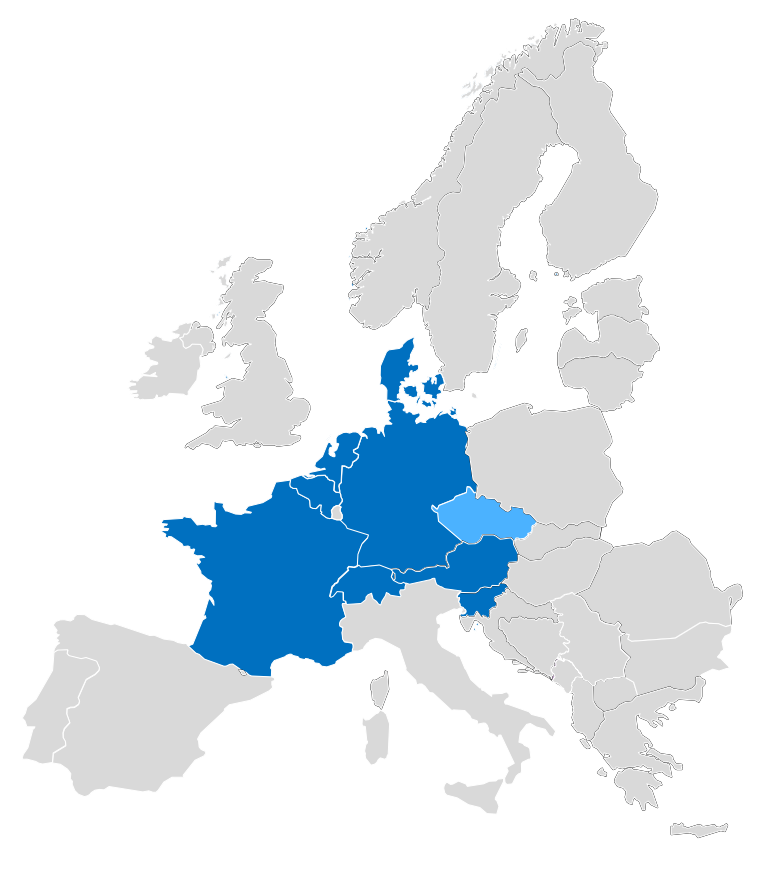
\includegraphics[page=1,trim=70 70 70 120, clip, width=0.4\textwidth]{./anhang/frc-map.png}
				\caption{Mitglieder der ENTSO-E für PRL \cite{ENTSO-E_PRL}}
				\label{Abb. Mitglieder ENTSO-E}
			\end{wrapfigure} des Verbundnetzes ermittelt.
			Um schnell und frequenzabhängig Strom einzuspeisen oder zu speichern, wird am Ort des Anbieters die Netzfrequenz gemessen. 
			Innerhalb von \SI{30}{\second} muss die komplette Regelleistung abrufbar sein.
			Nach \num{15} Minuten wird die Primärregelreserve heruntergefahren und die Minutenreserve übernimmt, um neu auftretenden Störungen entgegenzuwirken.
			Der Regelbereich befindet sich dabei innerhalb des Regelbands und außerhalb des Totbands (s. Abb. \ref{Abb. Beispielhafte Darstellung der Regelenergie in Abhängigkeit der Netzfrequenz}).
			Ab einer Netzfrequenz von \SI{49,99}{\hertz} bzw. \SI{50,01}{\hertz} muss der Stromlieferant die Primärregelleistung hochfahren und bei einer Frequenz von \SI{49,8}{\hertz} bzw. \SI{50,2}{\hertz} \SI{100}{\percent} seiner angebotenen Leistung abrufen bzw. liefern können \cite{Primäreserve_NextKraftwerke}. 
			
%			\begin{table}[H]
%				\renewcommand*{\arraystretch}{1.75}
%				\centering
%				\caption{Merkmale der Primärregelleistung \cite{Regelleistung_NextKraftwerke}}
%				\label{Tab. Merkmale der Primärregellung}
%				\begin{tabular}{ll}
%					\hline
%					Regelenergieart & Primärregelleistung  \\ \hline
%					Bereitstellung durch & ENTSO-E  \\
%					Aktivierung & \makecell[l]{Frequenzgesteuert: \\ Eigenständige Messung/Eingriff vor \\ Ort durch Anbieter der PRL} \\
%					Volle Leistung & Innerhalb von 30 Sekunden \\
%					\makecell[l]{Abzudeckender Zeitraum \\ nach Störungsfall} & \num{0} bis \num{15} Minuten  \\
%					Vergütung & Leistungspreis  \\
%					Mindestangebotsgröße & Ab $\pm\SI{1}{\mega\watt}$ (symmetrisch) \\
%					Tägliche Produkte & \makecell[l]{Positiv und negativ: \\ \num{6} Zeitintervalle über \num{4} Stunden} \\ \hline
%				\end{tabular}
%			\end{table}
			
			Die Ausschreibung von Primärregelleistung erfolgt täglich für einen Erbringungszeitraum von 0:00 Uhr bis 24:00 Uhr am Folgetag.
			Angebotsabgabe erfolgt am Vortag bis 8:00 Uhr  \cite{regelleistungnet_PRL_Ausschreibung}.
			Die Auktion erfolgt online über die Internetseite regelleistung.net \cite{regelleistungnet_PRL_Ausschreibung}.
			Zuschlag bekommen diejenigen Anbieter, welche für den ÜNB am wirtschaftlichsten sind.
			Der Anbieter, welcher Angebot und Nachfrage deckt, legt den Leistungspreis für alle anderen bezuschlagten Teilnehmer fest ("`Marginal Pricing"').
			In Abbildung \ref{Abb. Eigenschaften der drei Regelleistungsstufen} sind die wichtigsten Eckpunkte der Primärregelleistung dargestellt.		

		\subsubsection{Sekundärregelreserve}		
			
			Bei länger anhaltender Frequenzabweichung wird die Sekundärregelreserve (SRL) zugeschaltet, um die Frequenz durch sowohl positive als auch negative Regelleistung zu stabilisieren.
			Sie wird durch den innerhalb der Regelzone zuständigen Übertragungsnetzbetreiber per Signal angefordert und durch die an der Auktion teilgenommenen Anbieter von SRL abgerufen. 
			Die SRL wird nach \num{30} Sekunden zugeschaltet und muss nach fünf Minuten volle Regelarbeit liefern können. 
			Diese muss dann anschließend bis maximal eine Stunde nach Beginn des Störungsfalls geliefert werden. 
			Für den täglichen Abruf der Reserve gibt es sechs Zeitscheiben mit je vier Stunden.
			Da die Sekundärregelleistungsanbieter ihre Anlagen im Verbund nicht auf einige \si{\mega\watt} modulieren können, besteht fast kontinuierlicher Bedarf an Sekundärregelleistung.
			Durch den Netzregelverbund (NRV) wird ineffizientes "`Gegeneinanderregeln"' vermieden und die Höhe der vorzuhaltenden Regelleistung reduziert.
			Dieser wurde nach Aussagen der BNetzA auf weitere Nachbarstaaten ausgeweitet und trägt damit einer weiteren Reduzierung bei \cite[S. 207 f.]{Monitoringbericht_BNetzA}. \\
			
			Die Mindestangebotsgröße beträgt \SI{5}{\mega\watt}.
			Jedoch können nach einer Änderung des Beschlusses "`zur Festlegung von Ausschreibungsbedingungen und Veröffentlichungspflichten für Sekundärregelung"' der BNetzA auch Angebote in Höhe von \SI{1}{\mega\watt} bis \SI{4}{\mega\watt} eingereicht werden.
			Diese Änderung ist an die Maßgabe geknüpft, dass die Anbieter ausschließlich ein Angebot je Zeitscheibe für positive oder negative Regelleistung abgeben dürfen \cite{Beschluss_SRL}.
			Die Reduzierung erleichtert den Eintritt für kleinere Anbieter oder virtuelle Kraftwerke, welche mehrere Anlagen poolen.
			Pooling bezeichnet das Zusammenschalten, meist zu virtuellen Kraftwerken, von mehreren kleinen Anlagen zur Stromerzeugung oder -speicherung. \\
			
			Die Sekundärregelreserven werden täglich ausgeschrieben. 
			Bis zum Vortag um 9:00 Uhr muss das Angebot für den Folgetag abgegeben werden \cite{regelleistungnet_PRL_Ausschreibung}.
			Vergütet wird aufgeteilt nach dem Leistungs- und Arbeitspreis.
			Dies bedeutet, dass jeder Anbieter einen Festpreis für die Vorhaltung der angebotenen Leistung abgibt, egal ob diese abgerufen wird (Handel auf dem Regelleistungsmarkt).
			Der abgegebene Arbeitspreis wird auf dem Regelarbeitsmarkt gehandelt und gibt an, wie hoch die Vergütung je erbrachter \si{\mega\watt\hour} ist.
			Die Vergabe erfolgt nach einer Merit-Order-Liste, in welcher die Bieter nach aufsteigendem Preis aufgelistet werden.
			Jedoch erfolgt die Vergütung nach dem Pay-as-Bid Verfahren.
			Dies bedeutet, dass ausschließlich der angebotene Preis bezahlt wird \cite[S. 81 ff.]{Doktorarbeit_Reitsam}.
			Die Abbildung \ref{Abb. Eigenschaften der drei Regelleistungsstufen} zeigt nochmals die wichtigsten Eckdaten der Sekundärregelreserve. 
			\clearpage			
%			\begin{table}[H]
%				\centering
%				\caption{Merkmale der Sekundärregelreserve \cite{Regelleistung_NextKraftwerke}}
%				\label{Tab. Merkmale der Sekundärregelreserve}
%				\begin{tabular}{ll}
%					\hline
%					Regelenergieart &  Sekundärregelreserve  \\ \hline
%					Bereitstellung durch  & ÜNB  \\
%					Aktivierung & \makecell[l]{Durch verantwortlichen ÜNB \\ - manuelle Anforderung durch ÜNB} \\
%					Volle Leistung & Innerhalb von 5 Minuten \\
%					\makecell[l]{Abzudeckender Zeitraum \\ nach Störungsfall} & ab 30 Sekunden bis 1 Stunde \\
%					Vergütung &  Leistungs- und Arbeitspreis \\
%					Mindestangebotsgröße & \SI{5}{\mega\watt} positiv oder negativ\parnote{Eine Angebotshöhe von \SI{1}{\mega\watt} bis \SI{4}{\mega\watt} ist zulässig, sobald ein Anbieter von Minutenreserve nur ein einziges Angebot je Zeitscheibe für positive oder negative MRL in der jeweiligen Regelzone abgibt.}\\
%					Tägliche Produkte & \makecell[l]{Positiv und negativ: \\ \num{6} Zeitintervalle über \num{4} Stunden} \\ \hline
%				\end{tabular}
%				\parbox{0.7\textwidth}{\parnotes}
%			\end{table}
	
		\subsubsection{Minutenreserve}
		
			Die Minutenreserve ist die dritte Maßnahme zur Stabilisierung der Netzfrequenz. 
			Falls die Sekundärregelreserve die Frequenz nicht binnen \num{15} Minuten stabilisieren kann, muss die Minutenreserve innerhalb von weiteren \num{15} Minuten auf volle Leistung hochfahrbar sein.
			Die Mindestangebotsgröße beträgt wie bei der Sekundärregelreserve \SI{5}{\mega\watt} und unter der bereits erläuterten Prämisse können auch Angebote in Höhe von mindestens \SI{1}{\mega\watt} bis \SI{4}{\mega\watt} abgegeben werden.
			Das Pooling von Anlagenleistung ist ebenfalls möglich, um kleinerer Anbieter den Einstieg zu erleichtern.
			Geboten wird ebenfalls auf sechs Zeitscheiben, welche sich über jeweils vier Stunden erstrecken \cite[S. 81 ff.]{Doktorarbeit_Reitsam}. \\
			
			Die Vergütung erfolgt analog zu der Sekundärregelreserve, aufgeteilt nach Leistungs- und Arbeitspreis.
			Das Einreichen von Angeboten und die darauffolgende Vergabe verläuft ebenfalls analog zu der SRL.
			Die Angebotsabgabefrist verschiebt sich lediglich um eine Stunde  auf 10:00 Uhr \cite{regelleistungnet_PRL_Ausschreibung}.
			
			\begin{figure} [H]
				\centering
				\includegraphics[page=23,trim=40 340 40 130, clip, width=0.95\textwidth]{./anhang/Studie Tabelle Regelleistungen.pdf}
				\caption{Eigenschaften der drei Regelleistungsstufen \cite[S. 20]{Studie_Regelleistung_Wasserkraft}}
				\label{Abb. Eigenschaften der drei Regelleistungsstufen}
			\end{figure}
			\clearpage
	
%			\begin{table}[H]
%				\centering
%				\caption{Merkmale der Minutenreserve \cite{Regelleistung_NextKraftwerke}}
%				\label{Tab. Merkmale der Minutenreserve}
%				\begin{tabular}{ll}
%					\hline
%					Regelenergieart  & Minutenreserve \\ \hline
%					Bereitstellung durch & ÜNB \\
%					Aktivierung & \makecell[l]{Durch verantwortlichen ÜNB \\ - löst automatisch PRL ab}\\
%					Volle Leistung & Innerhalb von 15 Minuten \\
%					\makecell[l]{Abzudeckender Zeitraum \\ nach Störungsfall} & ab 5 Minuten bis 60 Minuten \\
%					Vergütung & Leistungs- und Arbeitspreis \\
%					Mindestangebotsgröße & \SI{5}{\mega\watt} positiv oder negativ\parnote{Eine Angebotshöhe von \SI{1}{\mega\watt} bis \SI{4}{\mega\watt} ist zulässig, sobald ein Anbieter von Minutenreserve nur ein einziges Angebot je Zeitscheibe für positive oder negative MRL in der jeweiligen Regelzone abgibt.} \\
%					Tägliche Produkte & \makecell[l]{Positiv und negativ: \\ \num{6} Zeitintervalle über \num{4} Stunden} \\ \hline
%				\end{tabular}
%				\parbox{0.7\textwidth}{\parnotes}
%			\end{table}
			\renewcommand*{\arraystretch}{1.5}
		
		\subsubsection{Primärenergieträger und Einsatzzeiten}
			
			Aus Tabelle \ref{Tab. Übersicht der Präqualifizierten Leistung je PrimärenergieträgerKategorie in Deutschland} können die präqualifizierten Leistungen je Primärenergieträger entnommen werden.
			Auffällig ist der hohe Anteil an Wasserkraft mit \SI{69,0}{\percent}, \SI{64,3}{\percent} und \SI{42,3}{\percent} an der Primär-, Sekundärreserve bzw. Minutenreserve.
			Dies ist auf die zügige Regelbarkeit von Wasserkraftwerken zurückzuführen.
			Hierbei findet jedoch keine Unterteilung in Laufwasser- oder Pumpspeicherkraftwerke statt.
			Da die Ausschreibung der Reserven täglich stattfindet, finden saisonale Schwankung der Wasserkraft dennoch Berücksichtigung \cite[S. 80]{Doktorarbeit_Reitsam}. 
			Außerdem kann festgestellt werden, dass die kontrahierte Leistung an Wasserkraft die in Deutschland installierte Leistung übersteigt.
			Dies ist im Wesentlichen auf zwei Punkte zurückzuführen.
			Zum einen bieten die Betreiber die Ein- sowie Ausspeicherung von Energie gemeinsam für die positive sowie negative Regelleistung an.
			Somit taucht die kumulierte Leistung aus Ein- und Ausspeicherung in der Tabelle auf.
			Zum anderen werden auch grenznahe Kraftwerke für die Bereitstellung von PRL kontrahiert \cite[S. 144]{Bericht_Wasserkraft}. \\
			
			Obwohl Erdgaskraftwerke schnell geregelt und hochgefahren werden können, weisen diese erst ab der Sekundärreserve nennenswerte Anteile auf (SRL: \SI{15,1}{\percent} und MRL: \SI{21,1}{\percent}).
			Für die Bereitstellung von Primärregelreserve muss das Kraftwerk bereits am Netz sein, um innerhalb von \num{30} Sekunden nennenswerte Regelleistung bereitstellen zu können (vgl. Kap. \ref{sect: Primärregelreserve}). 
			Wie bereits in Kapitel \ref{sect: Wie funktioniert der deutsche Strommarkt?} erläutert, liegen die Gaskraftwerke häufig an der Grenze zwischen Teilnahme und Nichtteilnahme am Strommarkt.  
			Wenn diese aufgrund von erhöhter Einspeisung der Erneuerbaren nicht am Strommarkt teilnehmen, können die Erdgaskraftwerke keine Primärregelleistung bereitstellen. \\
			
			Konventionelle Braun- und Steinkohlekraftwerke haben lediglich an der Minutenreserve einen größeren Anteil mit \SI{21,5}{\percent} (Braun- und Steinkohlekraftwerksleistung addiert).
			Die vorgehaltene Leistung steigt mit der Regelenergieart stetig an.
			Dies liegt wiederum an der mangelnden Schnelligkeit zur Regelung von Kraftwerksleistung. 
			Des Weiteren ist gut zu erkennen, dass Windkraft, Batteriespeicher und Demand-Side-Management Systeme keine großen Anteile an der Netzfrequenzstabilisierung aufweisen. 
			Bei Batteriespeichern liegt das an den massiven Investitionskosten für große Kapazitäten. 
			Jedoch kommt Batteriespeichern in Zukunft eine größere Rolle zu, da diese schnell viel Leistung speichern sowie abgeben können.
			Somit kann dem schrittweisen Wegfall der Momentanreserve ein Stück weit entgegengewirkt werden. 
			
			\begin{table}[H]
				\renewcommand*{\arraystretch}{1.2} %höhere Zeilen in tabellen
				\centering
				\caption{Präqualifizierte Leistung je Primärenergieträger/Kategorie in Deutschland, Stand: 01.01.2022 \cite{regelleistungnet_PRL_Ausschreibung}}
				\label{Tab. Übersicht der Präqualifizierten Leistung je PrimärenergieträgerKategorie in Deutschland}
				\begin{tabular}{lrrrrr}
					\hline
					\makecell[c]{Technologie \\ $\left[-\right]$} & \makecell[c]{FCR \\ $\left[\si{\giga\watt}\right]$}  & \makecell[c]{aFRR$+$ \\ $\left[\si{\giga\watt}\right]$} & \makecell[c]{aFRR$-$ \\ $\left[\si{\giga\watt}\right]$} & \makecell[c]{mFRR$+$ \\ $\left[\si{\giga\watt}\right]$} & \makecell[c]{mFRR$-$ \\ $\left[\si{\giga\watt}\right]$} \\ \hline
					Kernenergie & 0,22 & 0,18 & 0,19 & 1,27 & 1,27 \\
					Braunkohle & 0,56 & 1,20 & 1,21 & 4,16 & 4,20 \\
					Steinkohle & 0,48 & 1,05 & 1,07 & 2,98 & 2,88 \\
					Erdgas & 0,35 & 3,53 & 3,57 & 7,10 & 6,94 \\
					Öl & - & 0,26 & 0,03 & 1,28 & 0,09 \\
					Biogas/-masse & 0,04 & 1,82 & 2,29 & 2,27 & 2,75 \\
					Wasser & 4,79 & 15,10 & 15,15 & 13,99 & 14,01 \\
					Batteriespeicher & 0,48 & 0,08 & 0,06 & - & - \\
					Nachfrage/DSM & 0,02 & 0,12 & 0,07 & 0,20 & 0,14 \\
					Windkraft & - & - & 0,03 & - & 0,22 \\
					Sonstige & - & 0,01 & 0,01 & 0,11 & 0,30 \\ \hline
					Summe & 6,94 & 23,35 & 23,68 & 33,36 & 32,80
				\end{tabular}
				\renewcommand*{\arraystretch}{1.3} %höhere Zeilen in tabellen
			\end{table}
			\renewcommand*{\arraystretch}{1.3} %höhere Zeilen in tabellen
			
			Um die Diversität der Teilnehmer am Regelleistungsmarkt zu analysieren, kann die von den ÜNB veröffentliche Liste genutzt werden \cite{regelleistungnet_PRL_Ausschreibung}.
			Auf der Liste sind insgesamt \num{53} Unternehmen aufgeführt, welche am Regelleistungsmarkt ihre Kapazitäten zur Verfügung stellen.
			Ausschließlich Unternehmen, welche die Präqualifikationskriterien des in der Regelzone verantwortlichen ÜNB erfüllen, dürfen am Regelleistungsmarkt teilnehmen.
			Die Mehrzahl der aufgelisteten Marktteilnehmer sind Energieversorgungsunternehmen oder solche, die sich auf Energie- und Systemdienstleistungen spezialisiert haben.
			Lediglich acht Unternehmen sind aus der Industrie.
			Nennenswert ist der Ludwigshafener Chemiekonzern BASF oder Trimet Aluminium SE.
			Die aufgelisteten Industriekonzerne bieten in erster Linie Sekundär- und Minutenreserve an.
			Die wenigen Industrieunternehmen, die Primärreserven vorhalten, haben sich auf Batteriespeicher spezialisiert und können damit schnelle bzw. dynamische Reserven zur Verfügung stellen.
			Nach Stand vom 28.01.2022 haben 30 Unternehmen Primärregelleistung und jeweils 34 Sekundärregelleistung bzw. Minutenreserve angeboten. \\
			
			Aus dem Monitoringbericht der BNetzA geht hervor, dass die Primärregelreserven ständig und unmittelbar abgerufen werden. 
			Es findet also eine ständige Korrektur der Netzfrequenz statt.
			Ähnlich verhält es sich bei der Sekundärregelleistung. 
			In nahezu jeder der jährlichen \num{35040} Viertelstunden kommt die Sekundärregelreserve zum Einsatz.
			Im Hinblick auf die Minutenreserve kann ein deutlicher Rückgang zum Vorjahr verzeichnet werden (2019: 8313 und 2020: 3230) \cite[S. 213 ff.]{Monitoringbericht_BNetzA}.
			Auffallend ist ebenso, dass die positive MRL deutlich häufiger als die negative abgerufen wird (s. Tab. \ref{Tab. Abrufen von Minutenreserve}).
			Dies lag unter anderem am Mischpreisverfahren, dass von Oktober 2018 bis Juli 2019 in Kraft war.
			Durch vorrangiges Ansteigen der Leistungspreise zur Bereitstellung von Regelleistung sind die Arbeitspreise gesunken, welche nur bei einem Abruf von Regelenergie gezahlt werden.
			Demnach ergaben sich wenig Anreize für Bilanzkreisverantwortliche, ihre Netzprognosen sorgfältig abzugeben, da die bei Ungleichgewichten gezahlten Arbeitspreise zur aktiven Regulierung der Netzfrequenz sehr gering ausfielen.
			Somit war es wirtschaftlicher Angebot und Nachfrage über Aktivierung von Regelreserven als durch sorgfältige Verbrauchsprognosen zu regulieren \cite[S. 215 f.]{Monitoringbericht_BNetzA}.
						
			\begin{table}[H]
				\centering
				\caption{Einsatzhäufigkeit von positiver und negativer Minutenreserve \cite[S. 213 ff.]{Monitoringbericht_BNetzA}}
				\label{Tab. Abrufen von Minutenreserve}
				\begin{tabular}{lrr}
					\hline
					Einsatzhäufigkeit & 2019 & 2020 \\ \hline
					MRL positiv & 5271 & 2256 \\
					MRL negativ & 3042 & 974 \\ \hline
				\end{tabular}
			\end{table}
							
		\subsubsection{Momentanreserve}
		
			Eine weitere Möglichkeit zur Frequenzstabilisierung stellt die Momentanreserve dar.
			Da die ÜNB keinen direkten Einfluss auf die Momentanreserve haben, ist sie im Sinne der klassischen Regelleistungen wie PRL, SRL und MRL keine Systemdienstleistung.
			Momentanreserven sind rotierende Schwungmassen aus z.B. Generatoren, welche intrinsisch auf die Netzfrequenz wirken.
			Die Momentanreserve greift noch vor der Primärregelleistung ein und wirkt dadurch unmittelbar auf das Netz, ohne das diese gezielt ab- oder zugeschaltet wird.
			Generatoren, die direkt an das deutsche Stromnetz angeschlossen sind, sind auf eine Netzfrequenz von \SI{50}{\hertz} eingestellt.
			Bei Frequenzabfall oder -anstieg drehen sich die Schwungmassen der Generatoren langsamer oder schneller und wirken der Frequenzabweichung dämpfend entgegen \cite{Gawlik}.		
			Um die Frequenz innerhalb des Regelbands zu halten, nutzen diese die gespeicherte kinetische, magnetische oder elektrische Energie \cite{Energiespeicher}.
			Bei Ausbau der erneuerbaren Stromerzeuger, allem voran Wind- und Sonnenenergie, sind unmittelbar abrufbare Momentanreserven für die Aufrechterhaltung der Stromversorgung von zentraler Bedeutung.
			Die dauerhaft vorzuhaltende Momentanreserve bemisst sich an einem maximalen Leistungssprung bzw. Lastabfall von \SI{3}{\giga\watt} \cite{Bericht_Momentanreserve}. \\
			
			Aufgrund des direkten Zusammenhangs zwischen dem mechanischen Moment und der elektrischen Leistung ändert sich die Rotationsgeschwindigkeit in Abhängigkeit der Netzfrequenz.
			Die rotierende Schwungmasse wirkt aufgrund ihrer Massenträgheit durch Aus- und Einspeichern von Rotationsenergie einer Änderung der Rotationsgeschwindigkeit entgegen \cite{Bericht_Momentanreserve}.
		
	\subsection{Kraftwerksreserven zur Reserveleistungsvorhaltung}
	
		\begin{figure} [H]
			\centering
			\begin{overpic}[width=0.5\textwidth]{./anhang/Karte Kraftwerke.pdf}%
				\put(200,45){\small Netzreserve}%
				\put(200,35){\small Kapazitätsreserve}%
				\put(200,25){\small Sicherheitsbereitschaft}%
			\end{overpic}
			\caption{Netz-,Kapazitätsreserven und Sicherheitsbereitschaft in Deutschland \cite{Excel_Kraftwerksliste}, Quelle: Eigene Darstellung}
			\label{Abb. Reserven Deutschland}
		\end{figure}
	
		Abbildung \ref{Abb. Reserven Deutschland} zeigt die deutschlandweite Verteilung von Kraftwerken der Netz-, Kapazitätsreserve sowie den Braunkohlekraftwerken der Sicherheitsbereitschaft.
		Die drei Arten der Reserveleistungsvorhaltung sind im Energiewirtschaftsgesetz gesetzlich verankert und gegenwärtige Rahmenbedingungen klar definiert.
		Anhand der Karte wird verdeutlicht, dass die Netzreserve vor allem in Süddeutschland präsent ist (orange Kennzeichnung).
		Die Gründe für die überaus starke regionale Konzentration im Süden werden in Kapitel \ref{sect: Netzreserve} eruiert.
		Die rot gekennzeichneten Kapazitätsreserven sind hauptsächlich im Norden Deutschlands zu finden.
		Die drei verbliebenen Braunkohlekraftwerke aus der Sicherheitsbereitschaft sind mit blauen Punkten gekennzeichnet.
	
		\subsubsection{Netzreserve} \label{sect: Netzreserve}
		
			In erster Linie stellt die Netzreserve den ÜNB zusätzliche Kraftwerkskapazitäten für den Redispatch zur Verfügung.
			Redispatch bezeichnet dabei die Maßnahme, einen netzseitigen Engpass auszugleichen und zwischenzeitlich auftretende Lastspitzen abzufedern.
			In den meisten Fällen wird diese Maßnahme mit dem Nord-Süd-Gefälle des Stromnetzes in Verbindung gebracht.
			Besonders massiv zeigt sich dieses Problem im Winterhalbjahr, da der allgemeine Strombedarf größer ausfällt.
			Die Windparks im Norden des Landes produzieren viel Strom, welcher unter anderem aufgrund des mangelnden Netzausbaus nicht von Nord nach Süd transportiert werden kann.
			Um diesen Engpässen entgegenzuwirken und ein Gleichgewicht herzustellen, werden im Norden konventionelle Kraftwerke heruntergefahren und im Süden mit gleicher Leistung hochgefahren (s. Abb. \ref{Abb. Reserven Deutschland}).
			So findet ein Ausgleich bzw. eine Entlastung des Stromnetzes über die Grenzen der Regelzonen hinweg statt \cite{Netz_Kapa_Reserve_NextKraftwerke}. \\
			
			Kraftwerke können auf zwei verschiedene Arten in die Netzreserve überführt werden.
			Zum einen durch die freie Kontrahierung von Anlagen im In- und Ausland.
			Zum anderen durch Ausweisung von vorläufig oder endgültig stillzulegenden Kraftwerken, welche zuvor von den ÜNB und der BNetzA als systemrelevant eingestuft werden und damit nach dem EnWG nicht still gelegt werden dürfen \cite{EnWG}. \\
			
			Die Höhe der bereitzustellenden Reserve wird anhand von Berechnungen der BNetzA und der jährlichen Systemanalyse der ÜNB ermittelt.
			Innerhalb der Berechnung werden Erzeugungsspitzen im Norden, Kraftwerksausfälle im Süden und Nichtverfügbarkeiten von Netzbetriebsmitteln gegenüber gestellt.
			Anschließend erfolgt die Ermittlung, welche Leistung im Süden unterhalb des \num{50,4} Breitengrades zugeschaltet werden muss, um Angebot und Nachfrage gesamtheitlich auszubalancieren.
			Für den Winter 2022/2023 ergibt sich daraus eine Reserveleistung von \SI{8,264}{\giga\watt} \cite{Bedarf_Netz_Kapa_Reserve}.
			Für den Betrachtungszeitraum 2023/2024 bestätigt die BNetzA die Reserveleistung in Höhe von \SI{5,361}{\giga\watt}, welche durch die Systemanalyse der ÜNB ermittelt wurde \cite{Bedarf_Netz_Kapa_Reserve}.		
			Die geplante Verringerung der Leistung ist an den fortlaufenden Netzausbau geknüpft und kann nur bei Einhaltung der Ausbauziele eingehalten werden. 
			In Tabelle \ref{Tab. Kraftwerke Netzreserve} sind nach Stand des 31.05.2022 alle Kraftwerke der Netzreserve aufgeführt. 
			Da lediglich \SI{7,48}{\giga\watt} von deutschen Kraftwerken bereitgestellt werden können, müssen zusätzliche ausländische Kraftwerkskapazitäten hinzugekauft werden. 
			
			\begin{table}[H]
				\centering
				\caption{Kraftwerke in der Netzreserve \cite{Excel_Kraftwerksliste}}			
				\label{Tab. Kraftwerke Netzreserve} 
				\begin{tabular}{lllr}
					\hline
					\makecell[c]{Kraftwerk \\ $\left[-\right]$} & \makecell[c]{Ort \\ $\left[-\right]$} & \makecell[c]{Energieträger \\ $\left[-\right]$} & \makecell[c]{Nettoleistung \\ $\left[\si{\mega\watt}\right]$} \\ \hline 
					Heizkraftwerk Altbach & Altbach & Steinkohle & \num{433} \\
					Bexbach & Bexbach & Steinkohle & \num{726} \\
					GT 11 \& GT 12 & Darmstadt & Erdgas & \num{93} \\
					Staudinger 4 & Großkrotzenburg & Erdgas & \num{622} \\
					Ingolstadt 3 und 4 & Großmehring & Heizöl & \num{772} \\
					HLB 5 und 6 & Heilbronn & Steinkohle & \num{250} \\
					KWM Block 3 & Hohenhameln & Steinkohle & \num{690} \\ 
					RDK 4S DT \& GT & Karlsruhe & Erdgas & \num{353} \\
					KW2 DT27 & Mainz & Erdgas & \num{250} \\
					GKM Block 7 & Mannheim & Steinkohle & \num{425} \\
					Kraftwerk Marbach & Marbach & Heizöl & \num{425} \\
					Heyden 4 & Petershagen & Steinkohle & \num{875} \\
					Weiher 3 & Quierscheid & Steinkohle & \num{656} \\
					UPM Schongau DKW T4 \& T5 & Schongau & Erdgas & \num{64} \\
					Irsching 3 & Vohburg & Heizöl & \num{415} \\
					Walheim Block 1 \& 2 & Walheim & Steinkohle & \num{244} \\
					Kraftwerk Thyrow & Zossen & Erdgas & \num{187} \\ \hline
					Summe &  &  & \num{7480} \\ \hline
				\end{tabular}
			\end{table}
			
			Die Vergütung erfolgt anhand der Kosten für die dauerhafte Herstellung der Betriebsbereitschaft (Betriebsbereitschaftskosten) und anhand eines Leistungs- und/ oder Arbeitspreises, falls diese vorher mit dem zuständigen ÜNB ausgemacht worden sind \cite{EnWG}.
			Die Ausweisung durch die BNetzA und ÜNB ist für 24 Monate bindend und kann bei erneuter Ausweisung um weitere 24 Monate verlängert werden.		
			Des Weiteren dürfen die Anlagen der Netzreserve auch an den Ausschreibungen der Kapazitätsreserve teilnehmen.
			Bei erfolgreicher Ausschreibung erfolgt die Vergütung ausschließlich anhand der Kapazitätsreserve.
			Auf Anordnung der ÜNB müssen die Kraftwerksbetreiber jedoch ihre angegebene Leistung innerhalb der Netzreserve an den aktuellen Bedarf anpassen.
			
			\begin{table}[H]
				\centering
				\caption{Einsätze der Netzreserve \cite[S. 158]{Monitoringbericht_BNetzA}}
				\label{Tab. Einsätze Netzreserve}
				\begin{tabular}{lrrrr}
					\hline
					& \makecell[c]{Tage \\ $\left[\si{\day}\right]$} & \makecell[c]{Einsatzdurchschnitt \\ $\left[\si{\mega\watt}\right]$} & \makecell[c]{Maximale Leistungsanforderung \\ $\left[\si{\mega\watt}\right]$} & \makecell[c]{Summe \\ $\left[\si{\mega\watt\hour}\right]$} \\ \hline
					Januar & \num{9} & \num{148} & \num{622} & \num{12832} \\
					Februar & \num{14} & \num{228} & \num{1145} & \num{41638} \\
					März & \num{8} & \num{121} & \num{342} & \num{10147} \\
					April & \num{14} & \num{183} & \num{872} & \num{31022} \\
					Mai & \num{22} & \num{232} & \num{930} & \num{85851} \\
					Juni & \num{24} & \num{246} & \num{560} & \num{95267} \\
					Juli & \num{20} & \num{208} & \num{912} & \num{58588} \\
					August & \num{19} & \num{226} & \num{745} & \num{71112} \\
					September & \num{21} & \num{297} & \num{990} & \num{71576} \\
					Oktober & \num{10} & \num{156} & \num{385} & \num{18324} \\
					November & \num{17} & \num{322} & \num{1049} & \num{95149} \\
					Dezember & \num{13} & \num{231} & \num{740} & \num{43569} \\ \hline
					Gesamt & \num{191} &  &  & \num{635074} \\ \hline
				\end{tabular}
			\end{table}
			
			Aus dem Monitoringbericht der BNetzA geht hervor, dass in 2020 an \num{191} Tagen insgesamt ca. \SI{635}{\giga\watt\hour} Strom aus Kraftwerken der Netzreserve erzeugt wurden \cite[S. 157 f.]{Monitoringbericht_BNetzA}.
			In den Monaten Februar und November sind dabei die größten Leistungen angefallen.
			Dies ist mit dem bereits angesprochenen Nord-Süd-Gefälle zu begründen.	
			Weiterhin finden in Sommermonaten erhebliche Kraftwerkseinsätze statt.
			Hierbei rückt nicht die maximal angeforderte Leistung in den Vordergrund sondern die erzeugte Menge Strom.
			In den Sommermonaten liegt dies unter anderem an der hohen PV-Einspeisung und dem damit erforderlichen regelzonenübergreifenden Bilanzausgleich.
		    
		\subsubsection{Kapazitätsreserve}
		
			Die Kapazitätsreserve stellt den ÜNB eine zusätzliche Möglichkeit zur Verfügung, weitere Leistungsreserven zu aktivieren.
			Dies geschieht, wenn trotz freier Preisbildung an der Strombörse keine Deckung von Angebot und Nachfrage erzielt wird.
			Der Abruf der Kapazitätsreserve geschieht zeitlich nach der Strombörse und den Systemdienstleistungen (Regelleistungen) zur Frequenzstabilisierung. 
			Laut dem BMWK werden die Kraftwerke gemäß der Anfahrtszeit bereits am Vortag aktiviert, sobald am Day-Ahead-Market kein markträumendes Ergebnis abzusehen ist \cite{Netz_Kapa_Reserve_NextKraftwerke}.
			Die Anlagen in der Kapazitätsreserve sollen, sofern sie in netztechnisch geeigneten Regionen liegen, ebenfalls an der Netzreserve teilnehmen (vgl. Gaskraftwerk Thyrow).
			Ab dem Winterhalbjahr 2020/2021 waren Kraftwerkskapazitäten mit einer Leistung von \SI{2}{\giga\watt} ausgeschrieben.
			Nach Stand vom 31.05.2022 wurden Kraftwerke mit einer kumulierten Leistung von \SI{1,263}{\giga\watt} kontrahiert (s. Tab. \ref{Tab. Kraftwerke Kapazitätsreserve}). 
			Die daraus resultierende Unterdeckung muss im Ernstfall durch zusätzliche ausländische Kraftwerke kompensiert werden. 
		
			\begin{table}[H]
				\centering
				\caption{Kraftwerke in der Kapazitätsreserve \cite{Excel_Kraftwerksliste}}
				\label{Tab. Kraftwerke Kapazitätsreserve}
				\begin{tabular}{lllr}
					\hline
					\makecell[c]{Kraftwerk \\ $\left[-\right]$} & \makecell[c]{Ort \\ $\left[-\right]$} & \makecell[c]{Energieträger \\ $\left[-\right]$} & \makecell[c]{Nettoleistung \\ $\left[\si{\mega\watt}\right]$} \\ \hline 
					Gasturbinenkraftwerk Ahrensfelde & Ahrensfelde & Erdgas & \num{148} \\
					Gaskraftwerk Emden & Emden & Erdgas & \num{52} \\
					Gaskraftwerk Landesbergen & Landesbergen & Erdgas & \num{56} \\
					Gersteinwerk F \& G & Werne & Erdgas & \num{820} \\
					Kraftwerk Thyrow & Zossen & Erdgas & \num{187} \\ \hline
					Summe &  &  & \num{1263} \parnote{Laut Netztransparenz.de wurden \SI{1086}{\mega\watt} kontrahiert. Der Unterschied zu der Angabe der BNetzA besteht in unterschiedlichen Aussagen zur Nettokraftwerksleistung und Nichtberücksichtigung der Dampfturbinen im Gersteinkraftwerk E \& F. Diese sind jedoch in der Excel-Liste der BNetzA als Kapazitätsreserve ausgewiesen \cite{Excel_Kraftwerksliste}.} \\ \hline
				\end{tabular}
				\parbox{0.95\textwidth}{\parnotes}
			\end{table}	
		
			Die Vergabe der Kapazitätsreserve erfolgt durch wettbewerbliche Ausschreibungsverfahren.
			Die Anlagen können mehrmals an der Ausschreibung teilnehmen und werden anschließend jährlich vergütet.
			Die dabei entstehenden Kosten werden auf die Netzentgelte umgeschlagen. 
			Folgende Kosten werden dabei berücksichtigt: 
			\begin{itemize}
				\item Kosten zur Vorhaltung der Anlage
				\item Kosten für Anfahrvorgänge innerhalb anderer gesetzlicher Vorschriften
				\item Kosten zur Instandhaltung
				\item Kosten für Nachbesserungen
				\item Kosten für den Eigenstromverbrauch der Anlage
				\item Kosten für den Werteverbrauch
			\end{itemize}
			Gesondert werden außerdem folgende Kosten vergütet:
			\begin{itemize}
				\item Kosten aus Einspeisungen, die innerhalb der Kapazitätsreserve oder Netzreserve angefordert wurden
				\item variable Instandhaltungskosten für Einspeisungen innerhalb der Netzreserve
				\item Kosten für die Sicherstellung der Brennstoffversorgung 
				\item Kosten, die durch weitere Anforderungen der ÜNB entstehen (um die Schwarzstartfähigkeit oder Blindleistungseinspeisung ohne Wirkleistungseinspeisung herstellen zu können)
			\end{itemize}
			Für die Ausschreibung vom 1. Oktober 2022 bis zum 30. September 2024 wird dabei ein Preis je Megawatt von \SI{62940}{\euro} aufgerufen.
		
		\subsubsection{Sicherheitsbereitschaft}
		
			Falls Netz- und Kapazitätsreserve nicht ausreichen, um Angebot und Nachfrage am Strommarkt zu decken, sieht das EnWG die Vorhaltung von Kraftwerksleistung innerhalb der Sicherheitsbereitschaft vor.
			Die Sicherheitsbereitschaft impliziert ausschließlich Braunkohlekraftwerke, welche aufgrund des Kohleausstiegs vorläufig stillgelegt werden sollen.
			Grund ist, dass Braunkohlekraftwerke für \SI{50}{\percent} der \COO-Emissionen im Stromsektor verantwortlich sind, dabei jedoch nur \SI{24}{\percent} der Erzeugung abdecken \cite[S. 11 u. S. 31 f.]{Agora_Braunkohle}.		
			Für die in Tabelle \ref{Tab. Kraftwerke Sicherheitsbereitschaft} aufgelisteten Kraftwerke wurden im Vorhinein Stilllegungstermine vereinbart.
			Nach §13g EnWG dürfen diese jedoch nicht vorläufig stillgelegt werden und stehen den ÜNB für weitere vier Jahre ab dem Stilllegungstermin zur Verfügung.
			Die Kraftwerke Buschhaus und Frimmersdorf sind nach der Sicherheitsbereitschaft endgültig stillgelegt worden \cite{EnWG}.  
			\begin{table}[H]
				\centering
				\caption{Kraftwerke in der Sicherheitsbereitschaft \cite{Excel_Kraftwerksliste}}
				\label{Tab. Kraftwerke Sicherheitsbereitschaft}
				\begin{tabular}{lllr}
					\hline
					\makecell[c]{Kraftwerk \\ $\left[-\right]$} & \makecell[c]{Ort \\ $\left[-\right]$} & \makecell[c]{Energieträger \\ $\left[-\right]$} & \makecell[c]{Nettoleistung \\ $\left[\si{\mega\watt}\right]$} \\ \hline 
					Niederaußem E \& F & Bergheim & Braunkohle & \num{594} \\
					Neurath C & Grevenbroich & Braunkohle & \num{292} \\
					Kraftwerk Jänschwalde Block E \& F & Jänschwalde & Braunkohle & \num{1000} \\ \hline
					Summe &  &  & \num{1886} \\ \hline
				\end{tabular}
			\end{table}
			Die Anlagen der Sicherheitsbereitschaft müssen innerhalb von zehn Tagen betriebsbereit sein.
			Nach erfolgreicher Betriebsbereitstellung muss nach elf Stunden Mindestleistung und weiteren 13 Stunden Volllast zur Verfügung stehen.
			Der Nachweis zur Einhaltung des gesetzlichen Zeitplans erbringen die Betreiber selbst.
			Eine unabhängige Prüfung seitens der BNetzA oder ähnlichen Institutionen erfolgt nicht.  
			Für die Vorhaltung der Kraftwerksleistung werden insgesamt 1,61 Milliarden Euro bereitgestellt und auf die Netzentgelte umgelegt \cite{Netz_Kapa_Reserve_NextKraftwerke}.
			Falls die Betreiber nicht rechtzeitig die versprochene Leistung bereitzustellen, sinkt die Vergütung.
			Nach 13 Tagen findet keine Vergütung mehr statt \cite{EnWG}. \\
			
			Die Linkspartei und Grünen haben zudem öffentlich Kritik an der Notwendigkeit und Einsatzbereitschaft der "`Braunkohlereserve"' geäußert.
			Zum einen wurde die fehlende unabhängige Beurteilung bzgl. des Zeitplans zur Betriebsbereitschaft bemängelt.
			Zum anderen wurde die Transportlogistik zur Brennstoffbeschaffung sowie die ungeregelte Personalverfügbarkeit kritisiert.
			Außerdem wurde angemerkt, dass vor Einsatz der Sicherheitsbereitschaft mehrere Mechanismen greifen, um zusätzliche Kraftwerksleistung zur Verfügung zu stellen.
			Eine weitere Reserve sei daraufhin nicht unbedingt notwendig \cite{Netz_Kapa_Reserve_NextKraftwerke}.
			
		
	\subsection{Veränderungen der Kraftwerksreserven aufgrund des russischen Überfalls auf die Ukraine}
	
		Aufgrund des Überfalls Russlands auf die Ukraine und den damit verminderten Gaslieferungen aus Russland soll der Anteil von Erdgas an der Stromproduktion reduziert werden.
		Hierfür sind zwei Verordnungen, basierend auf den Verordnungsermächtigungen im Energiewirtschaftsgesetz, die durch das Ersatzkraftwerkebereithaltungsgesetz beschlossen wurden, in Kraft getreten.
		Innerhalb dieser ist die reguläre Teilnahme am Strommarkt für die Braunkohlekraftwerke aus der Sicherheitsbereitschaft und Steinkohlekraftwerke aus der Netzreserve geregelt.
		Dafür gehen die Kraftwerke der Sicherheitsbereitschaft ab dem 01. Oktober in die neu geschaffene Versorgungsreserve über.
		Diese erlaubt eine reguläre Teilnahme am Strommarkt bis zum 30. Juni 2023.
		Die Rückkehr in den Strommarkt aus der Netzreserve gilt bis zum 31. März 2024.
		Bedingung für Inkrafttreten beider Verordnungen ist, dass die Alarmstufe Gas oder Notfallstufe Gas ausgerufen ist. 
		Die Betriebserlaubnis erlischt bei Aufhebung der Alarmstufe oder Notfallstufe Gas am Ende des darauffolgenden Quartals.
		Somit soll der Weiterbetrieb planbarer und wirtschaftlich attraktiver gestaltet werden.
		Dies wird in den Kapiteln zur aktuellen Bewertung der Kraftwerksreserven weitergehend ausgeführt. \\
		
%		In Folge der Verordnungen sind nach dem Stand vom 25.10.2022 zwei Steinkohlekraftwerke aus der Netzreserve wieder in den Strommarkt eingetreten.
%		Dies betrifft das Kraftwerk Mehrum in Hohenhameln mit einer Nettokraftwerksleistung von \SI{690}{\mega\watt} und das Kraftwerk Heyden 4 in Petershagen mit \SI{875}{\mega\watt}.
		
		
		
		
\clearpage
	